\section{Experimental Setup and Evaluation}

\begin{figure}[ht]
\includegraphics[width=\linewidth]{images/Topology.eps}
\caption{Topology used in the experiments.}
\label{fig:topo}
\end{figure}

We use mininet and Ryu controller for the experiments.
We are considering the topology given in the figure \ref{fig:topo}. C$_0$ is the remote controller, S1, S2, S3 are the three switches.
The flow is going from host h$_{2}$ to h$_{6}$.
Minimum and maximum polling time are set to be 0.5 seconds and 5 seconds respectively.
Which is same as CEMON \cite{CEMON}. 
In our experiment, we extend the polling component to poll in 2 parallel threads, for CEMON/Multi-Objective another for Curvature Based Sampling.
We have two applications of our algorithm 1st to measure total bytes of the flow, 2nd to measure utilization of the flow.
We use RMSE w.r.t. actual traffic as a measure of accuracy.
Overhead is defined as the number of stat request requests and responses.
We also define a cost function for the scheme to evaluate the tradeoff between cost and accuracy.
The measurement interval for utilization is 1 second.

\subsection{Cost function}
As overhead increases, cost decreases and vice versa. Though the decrease is not by the same amount.
We have to develop some measure to decide which scheme is better these cases for this we propose using a cost function.
The cost function for our scheme is defined as the product of Normalized cost and Overhead.
As either of the product or Overhead increase, the cost of the scheme increases.
This helps us to judge the cases where there is indecision just based on cost or overhead. 


% \subsection{Graphs}
% \begin{figure}[ht]
% 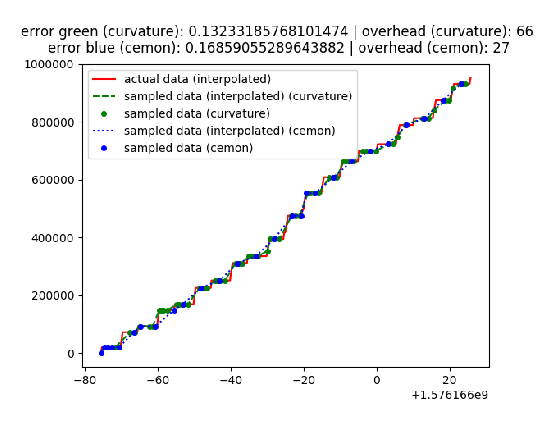
\includegraphics[width=\linewidth]{images/graphs/nrmse/br2_curvature_vs_cemon.eps}
% \caption{MPG | BR2 | NRMSE}
% \label{fig:br2}
% \end{figure}

% \begin{figure}[ht]
% 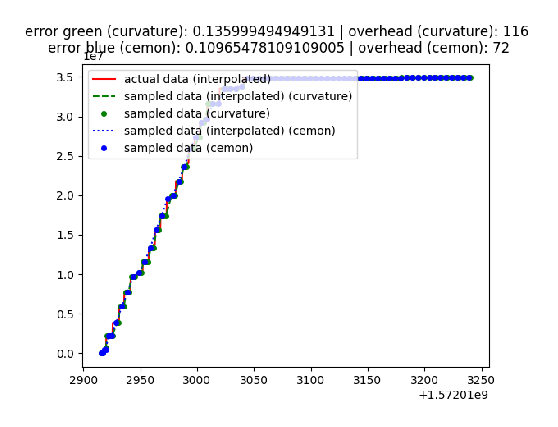
\includegraphics[width=\linewidth]{images/graphs/nrmse/matrix2_curvature_vs_cemon.eps}
% \caption{MPG | MATRIX2 | NRMSE}
% \label{fig:matrix2}
% \end{figure}

% \begin{figure}[ht]
% 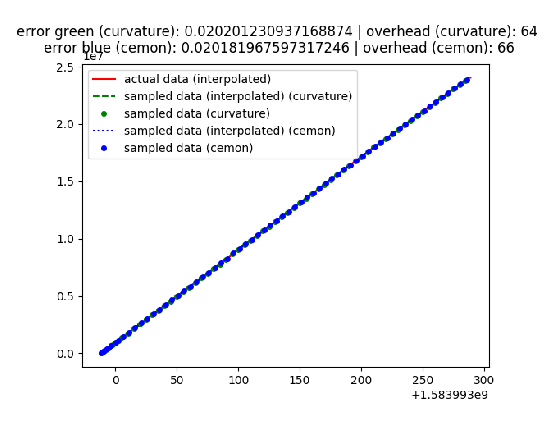
\includegraphics[width=\linewidth]{images/graphs/nrmse/pareto0.1_curvature_vs_cemon.eps}
% \caption{Pareto0.1 | NRMSE}
% \label{fig:pareto1}
% \end{figure}

% \begin{figure}[ht]
% 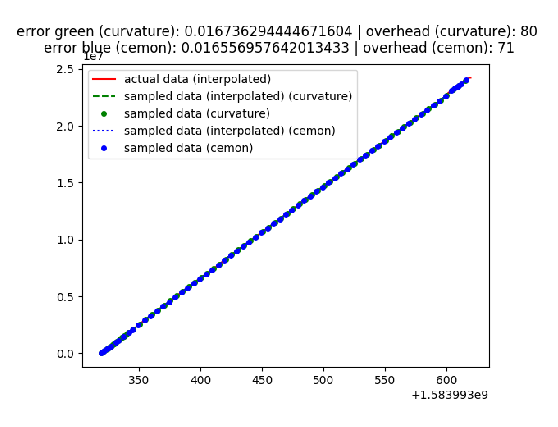
\includegraphics[width=\linewidth]{images/graphs/nrmse/pareto0.2_curvature_vs_cemon.eps}
% \caption{Pareto0.2 | NRMSE}
% \label{fig:pareto2}
% \end{figure}

% \begin{figure}[ht]
% 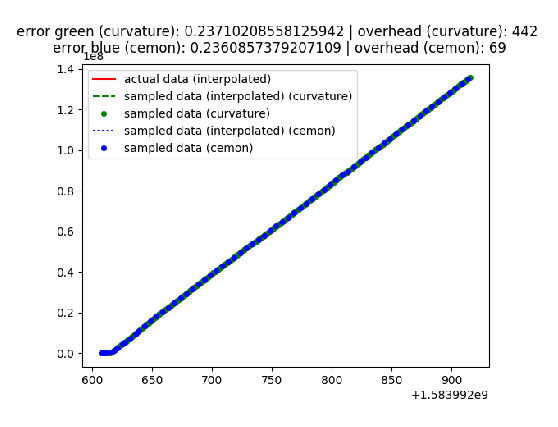
\includegraphics[width=\linewidth]{images/graphs/nrmse/poission0.1_curvature_vs_cemon.eps}
% \caption{Poisson0.1 | NRMSE}
% \label{fig:poisson1}
% \end{figure}

% \begin{figure}[ht]
% 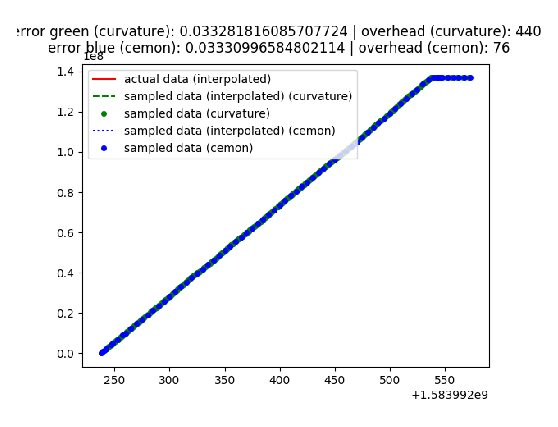
\includegraphics[width=\linewidth]{images/graphs/nrmse/poission0.2_curvature_vs_cemon.eps}
% \caption{Poisson0.2 | NRMSE}
% \label{fig:poisson2}
% \end{figure}

% \begin{figure}[ht]
% 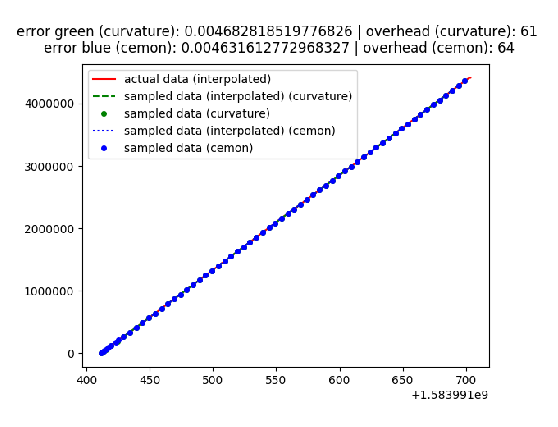
\includegraphics[width=\linewidth]{images/graphs/nrmse/voip0.1_curvature_vs_cemon.eps}
% \caption{VoIP0.1 | NRMSE}
% \label{fig:voip1}
% \end{figure}

% \begin{figure}[ht]
% 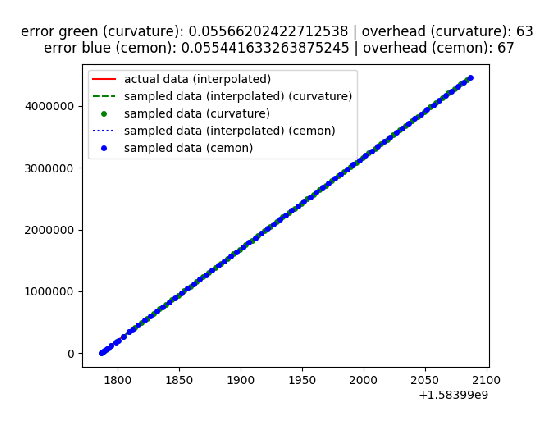
\includegraphics[width=\linewidth]{images/graphs/nrmse/voip0.2_curvature_vs_cemon.eps}
% \caption{VoIP0.2 | NRMSE}
% \label{fig:voip2}
% \end{figure}
